\section{Processamento de Sinais}

O estudo do processamento de sinais foi feito com base nas placas que vão captar as informações, pois os sistemas que se comunicam com elas são diferentes e podem ter diferentes implementações, logo, a equipe de processamento de sinais se baseou na definição a placa
pois os softwares que se comunicam com elas dependem das mesmas.

\subsection{Entendimento}

O projeto da equipe de processamento de sinais consiste no recebimento dos dados enviados pela placa \textit{NI 6320}, processamentos dos valores fornecidos e, por meio de uma interface gráfica de controle, dar ao operador a decisão de qual o comportamento o sistema deve tomar.

\subsection{Levantamento dos materiais}

É possível fazer a mesma operação de processamento de sinais com placas como:
\begin{itemize}
    \item Arduino
    \item Raspberry Pi
    \item NI 6320
    
\end{itemize}

A escolha da placa NI 6320, se da pelas facilitações para sistemas de arrefecimento, descritas em seu manual. Estas placas são indicadas para aplicações de controle a automação de medição. O que justifica a funcionalidade desejada no projeto a ser desenvolvido.

Abaixo segue uma tabela de comparação sobre as possibilidades a serem implementadas.

    \begin{table}[htb]
        \centering
        \begin{tabular}{|p{3cm}|p{3cm}|p{3cm}|p{3cm}|}
        \hline
        Critérios & Arduino Uno & Raspberry Pi 3 & NI 6320 \\ \hline
        Preço(R\$) & R\$ 116.68 & R\$ 112.50 & R\$ 2,470.00 \\ \hline
        Cliente já possui & Não Possui & Não Possui & Possui \\ \hline
        Implementação da solução & Construção completa da solução & Construção completa da solução & Software de apoio e fornecimento dos dados já implementados\\ \hline
        \end{tabular}
        \caption{Comparação dos materiais}
        \end{table}

\subsection{Verificação}

Mesmo com o preço da \textit{NI 6320} muito acima das outras opções, devido ao cliente já possuir um exemplar para uso e a placa possuir muitas facilidades para o tipo de projeto que será desenvolvido por possuir um conversor analógico-digital com uma boa resolução (12 bits/Sample) e uma taxa de amostragem de 250kS/s. A placa Raspberry não possui um conversor analógico-digital e o Arduino tem uma baixa frequência de operação. Logo a placa \textit{NI 6320} apresenta melhores opções para o projeto.
A placa \textit{NI 6320} também pode ser utilizada com o software \textit{LabView}, que facilita na implementação de soluções com as características presentes no projeto.

\newpage\begin{figure}[!htb]                                                               
    \centering                                                                      
    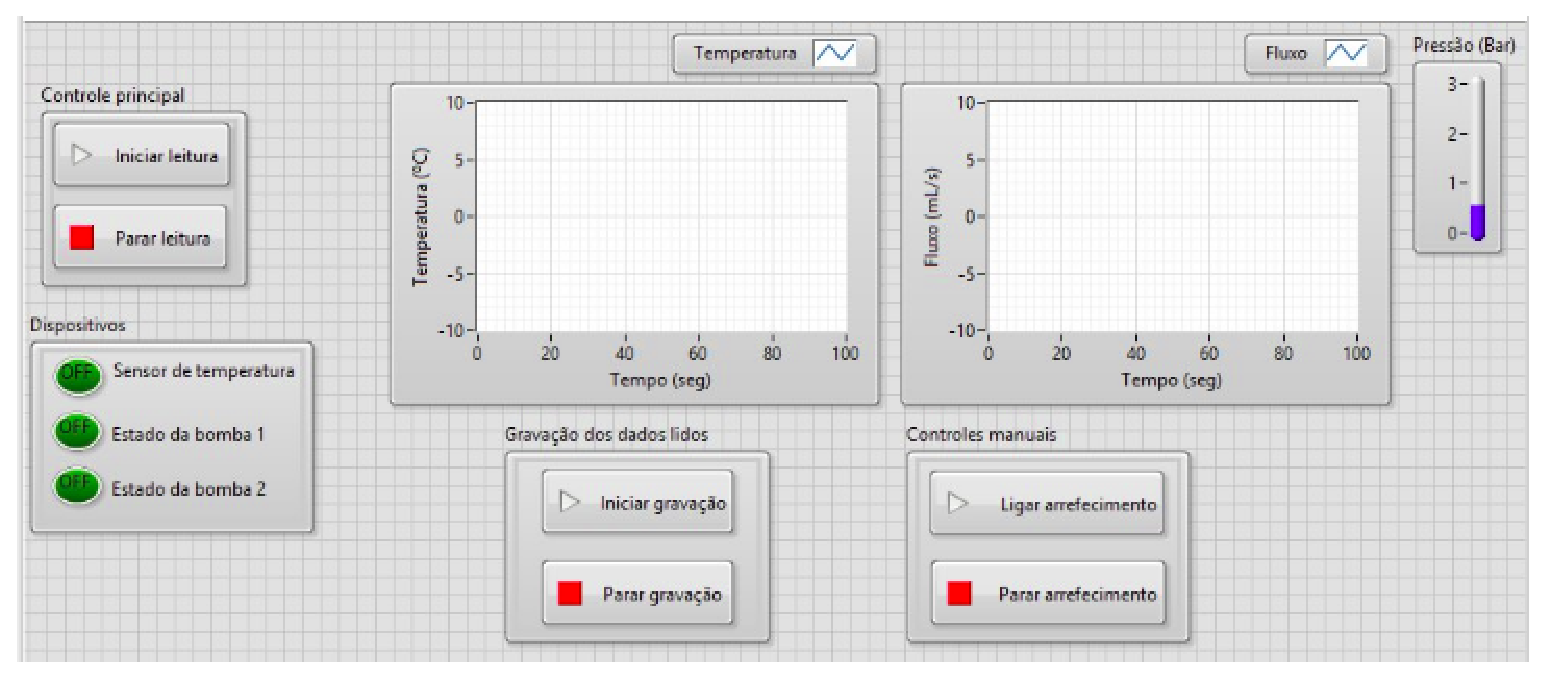
\includegraphics[scale=0.6, keepaspectratio=true]{figuras/labview_1.eps} 
    \caption{Imagem 1 - LabView}
 \end{figure}
 \begin{figure}[!htb]                                                               
    \centering                                                                      
    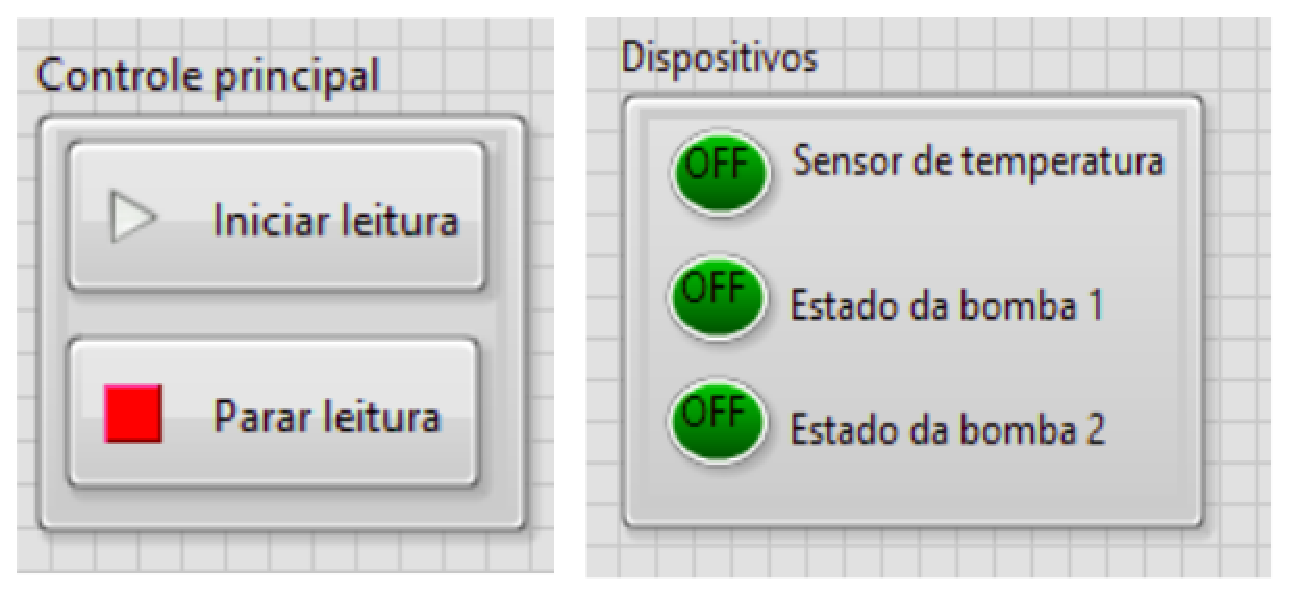
\includegraphics[scale=0.5, keepaspectratio=true]{figuras/labview_2.eps} 
    \caption{Imagem 2 - LabView}
 \end{figure}
 \begin{figure}[!htb]                                                               
    \centering                                                                      
    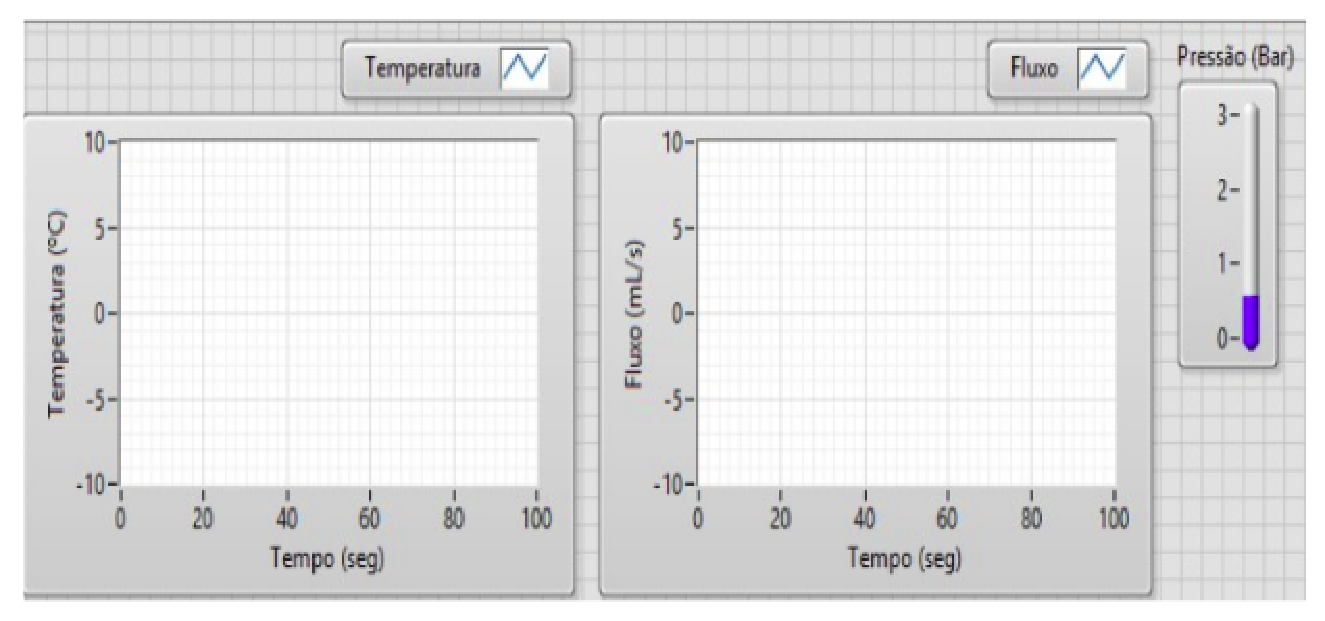
\includegraphics[scale=0.5, keepaspectratio=true]{figuras/labview_3.eps} 
    \caption{Imagem 3 - LabView}
 \end{figure}
 

\newpage\subsection{Riscos do processamento de sinal}
Abaixo esta o levantamento dos riscos da equipe de Processamento de Sinal.

\begin{table}[!htp]
    \centering
    \begin{tabular}{|p{1cm}|p{2cm}|p{2cm}|p{2cm}|p{2cm}|p{1.7cm}|p{2.9cm}|}
    \hline
    \textbf{ID}  & \textbf{Risco} & \textbf{Tipo de Risco} & \textbf{Descrição} & \textbf{Descrição do Impacto} & \textbf{Impacto} & \textbf{Probabilidade} \\ \hline
    R01 & Ruído no sinal & Técnico & O sinal sofre interferência por ruídos & Interferência por ruído no sinal gerado & Alto & Baixa \\ \hline
    R02 & Calibração incorreta do sensor & Técnico & O sensor não foi calibrado de forma correta & Sensor calibrado incorretamente gerando erros & Alto & Baixa \\ \hline 
    R03 &Erro de conexão entre o sensor e o conversor A/D &Técnico &O conversor A/D não recebe o sinal  transmitido pelo sensor &O conversor A/D não recebe o sinal  transmitido pelo sensor &Alto &Baixa \\ \hline
    R04 &Problema na placa de aquisição de dados &Técnico &A placa de aquisição de dados não funciona corretamente &A placa de aquisição de dados não funciona corretamente &Muito alto &Baixa \\ \hline
    R05 &Equipe não se adaptar a tecnologia labView &Técnico &Equipe não possuir conhecimento na área &Equipe não possuir conhecimento em labVIEW &Muito alto &Baixa \\ \hline
\end{tabular}
    \caption{Analise dos riscos de processamento de sinal}
    \end{table}

\newpage\subsection{Resposta aos riscos do processamento de sinal}
Abaixo esta descrito as respostas aos riscos levantados na tabela acima.

\begin{table}[h]
    \centering
    \begin{tabular}{|p{1cm}|p{2cm}|p{2cm}|p{2cm}|}
        \hline
        \textbf{ID}  & \textbf{Descrição} & \textbf{Ação} & \textbf{Prioridade} \\ \hline
        R01 &Ruído no sinal &Verificar causa do ruído e solucioná-lo & Média(10) \\ \hline
        R02 &Calibração incorreta do sensor &Calibrar o sensor de forma correta &Alta(18) \\ \hline
        R03 &Erro de conexão entre o sensor e o conversor A/D &Verificar local de erro da conexão e arrumá-lo &Alta(20) \\ \hline
        R04 &Problema na placa de aquisição de dados &Substituição da placa de aquisição de dados &Alta(25) \\ \hline
        R05 &Equipe não se adaptar a tecnologia labView &Treinamentos e dojos sobre a tecnologia &Alta(23) \\ \hline
    \end{tabular}
\caption{Reposta aos riscos de processamento de sinal}
\end{table}